\documentclass{article}
\usepackage{amsmath, amsfonts, amsthm, amssymb}  
\usepackage{secdot}
\usepackage{epsfig}
\usepackage{fancyvrb}
\usepackage{cprotect}
\usepackage[T1]{fontenc}
\usepackage{epstopdf}
\usepackage{url}
\usepackage{rotating}
\usepackage{graphicx}
\usepackage{caption}
\usepackage{subcaption}
\usepackage{multirow}
\usepackage{setspace}
\usepackage{array}
\usepackage{fancyhdr}
\usepackage{lastpage}
\usepackage[T1]{fontenc}

\usepackage{geometry}
\geometry{letterpaper, left=1in, right=1in, top=1in, bottom=1in}

\pagestyle{fancy}
\fancyhf{}
\rhead{\thepage/\pageref{LastPage}}
\lhead{OSU ECEN 2233 - Logic Design - Fall 2023}
\rfoot{\LaTeX}


% ----- Identifying Information -----------------------------------------------
\newcommand{\myassignment}{Project: Fun with Cellular Automata and HDMI}
\newcommand{\myduedate}{Assigned: Wednesday 11/8; Due \textbf{Friday 12/8} (midnight)}
\newcommand{\myinstructor}{Instructor: James E. Stine, Jr.}
% -----------------------------------------------------------------------------

\begin{document}
\begin{center}
  {\huge \myassignment} \\
  {\large \myduedate} \\
  \begin{flushright}
  \myinstructor \\
  \end{flushright}
\end{center}

\section{Introduction}

This project is meant to be an encompassing project that gives you the
full experience of all that you learned in this course.  It will bring
ideas that we covered as well as had within laboratories.  It will
also try to reinforce all the skills you learned during your time in
laboratory.

We will revisit using something completely different but in this setting we
will have an idea of what combinational and sequential digital systems
are.
The project involves something called cellular automata by using the Game of Life invented by
John Horton Conway in 1970~\cite{games1970fantastic}. Cellular automata uses discrete, abstract computation systems
that are proven useful in numerous complexity models as even more advanced dynamic system
over many scientific fields. This field is extremely exciting in that it utilizes computation in
some form to model repetitive systems to accomplish an outcome.  Much
of the ideas on cellular automata are intertwined within new ideas on
artificial intelligence and machine learning.

The game works by giving an initial matrix and then the game repeatedly creates multiple
matrices after processing the data. Since the game works by itself based on an initial grid matrix,
it is sometimes called a zero-player game. The game works by computing a two-dimensional
grid of square cells. Currently, the game is only designed for an
$8 \times 8$ matrix, however, it can
easily be expanded to larger sizes. Every cell interacts with its nearest neighbor
that is horizontal, vertical, and diagonally adjacent to each cell in
the grid (sometimes called a
Moore Neighborhood). At each iteration, several rules are utilize based on whether the grid is
alive (bit=1) or dead (bit=0). The rules are, as follows~\cite{CleveMolerLife}:
\begin{enumerate}
  \item Any live cell with fewer than two live neighbors dies, as if caused by under-population.
  \item Any live cell with two or three live neighbor’s lives on to the next generation.
  \item Any live cell with more than three live neighbors dies, as if by overcrowding.
  \item Any dead cell with exactly three live neighbors becomes a live
    cell, as if by reproduction.
\end{enumerate}
To make the matrix easier to use, the grid is only populated with a $1$ or a $0$ for alive and dead,
respectively. The initial pattern for the matrix is called a seed of the system and it determines the
patterns that each iteration produces. Each generation is subsequently computed by the rules
given and based on the seed interesting outcomes possibly emerge. For more information, please
consult the WikiPedia page at the following URL:
\url{http://en.wikipedia.org/wiki/Conway%27s_Game_of_Life}.  

\section{Background}

The implementation uses a simple register to hold the size of the grid space. For example, the
default implementation is given for a $8 \times 8$ matrix, as shown in
Figure~\ref{conway-grid}, therefore, the register
size will be allocated for 64 bits where each bit determines whether a specific grid is alive or
dead. Larger matrices can easily be created by expanding the register size, however, special
attention has to be made when accessing a specific grid point. For example, if a user wants to
target (row = 4) and (column = 5) of the matrix, the grid point will
be given by: $(4-1)*8 + (5-1) = 28$. Each row and column is subtracted
by $1$, since the starting grid point at the upper left hand
corner is $(0,0)$.
\begin{figure}
  \centering
  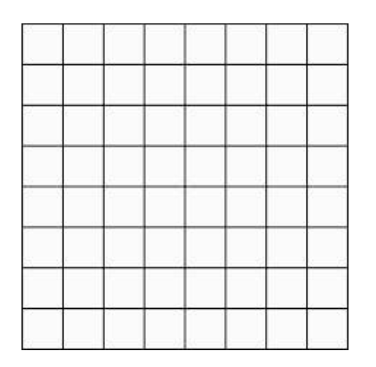
\includegraphics[scale=0.4]{grid8x8.png}
  \caption{Default 8 x 8 Conway Game of Life Matrix}
  \label{conway-grid}
\end{figure}

An $8 \times 8$ grid looks something like Figure~\ref{conway-grid}
where each grid can contain a $0$ or $1$ indicating that
spot is either dead or alive, respectively. Again, the top left-hand portion of the grid is $(0,0)$.
Although $8 \times 8$ is rather small, the matrix can easily be expanded, if necessary by examining the
datpath Verilog code. A sample Conway game of life is shown at the
following URL:
\url{http://pmav.eu/stuff/javascript-game-of-life-v3.1.1/}. 

As stated previously, the matrix is held in a register based on the number of columns and rows.
For example, a register in Table~\ref{matrix4x4} is shown for a
$4 \times 4$ matrix. The key to using the matrix is
making sure that a new matrix (called an evolving matrix) accesses the register based on several
points, as expressed previously.
\begin{table}
  \centering
  \begin{tabular} {|c|c|c|c|c|c|c|c|c|c|c|c|c|c|c|c|c|c|c|c} \hline
    0 & 1 & 2 & 3 & 4 & 5 & 6 & 7 & 8 & 9 & 10 & 11 & 12 & 13 & 14 &
    15 \\ \hline \hline
    1 & 0 & 1 & 1 & 0 & 0 & 1 & 1 & 1 & 1 & 1 & 1 & 0 & 0 & 0 & 0 \\ \hline
  \end{tabular}
  \caption{Sample Register for a 4 x 4 Matrix}
  \label{matrix4x4}
\end{table}

The initial matrix is called the seed matrix and many interesting patterns can be generated based
on different seeds. You can search the Internet for some good seeds. I used the following seed
to test the design and you are welcome to use the same seed for your testing (given as a Verilog
statement) as shown in Figure~\ref{starting-seed}:
\begin{figure}
\begin{Verbatim} [frame=single]
  assign grid = 64'h0412_6424_0034_3C28;
\end{Verbatim}
\caption{Good Starting Seed for Conway's Game of Life}
\label{starting-seed}
\end{figure}

The key to digital systems is that digital logic can process data in parallel. To help you with your
project, I have coded up the project datapath in Verilog to show how this works. The baseline
project involves two simple modifications to complete the project: adding the control logic and
adding logic to display to a VGA screen.
In order to complete this project, the following items must be
functional on the board:
\begin{itemize}
\item Control logic should be added to control each iteration of the
  zero-player game.
\item A video system in order to handle output to a screen through HDMI.
\item All testbenches for the system, control, and datapath.
\item Cleaned up code removing any unnecessary logic and/or states.
\item A report documenting the complete game and its operation.
\item Anything you can think of to promote your project!
\end{itemize}

This project is not difficult and it is an excellent choice for groups that want a straightforward
project and/or who wish to spend a minimal amount of time as possible on the project. However,
it is in your best interest to make the project better! Any modification beyond the baseline
project will incur extra points that could help compensate for a bad test, missing homework, or
bad quiz. The following are potential modifications you can easily add
for extra credit:
\begin{itemize}
\item Add some cool patterns (e.g., gliders, spaceship – check Internet for good starting seeds)
\item Mutations/Variations on Life (add extra rules $\rightarrow$ sometimes called better CA)
\item Make code easier to adapt size (matrix grid)
\item $2$-dimensional – with color.
\item Add poster to explain to masses!
\item Create a YouTube® channel on this!
\item Add music by attaching speakers (ask TA) to output music something is
  happening.
\end{itemize}

\section{Implementation}

The basic idea for the inputs and output includes your move which you
should add through the switches.  You will technically only need a
``Start'' switch to get things going.  The output of the datapath
should go to the HDMI section.  The controller for the HDMI will be
given to you, but you will be required to figure out how to display on
it the screen (with help of course).

The main key elements of the design will be provided to you, such as
the \verb!evolve! and \verb!rules!
modules.  But, you will have to add registers,
control logic (e.g., Finite State Machines), multiplexors, input/output signals.
It is advisable to use as many input/output signals to help you debug
what is going on as you simulate and get to your final
implementation.

You should use many of the elements discussed in our
textbook~\cite{ddca-riscv}.  I would highly advise using the
\textit{idioms} we discussed in class 
and in the textbook for things
like registers making sure that you also reset or enable them appropriately.
That is, you should also incorporate a \textbf{reset} somewhere into your
design.  All of the HDL discussed in the textbook~\cite{ddca-riscv} is
on Canvas as a zip file.  Feel free to use this HDL in any way you wish.

HDMI or High-Definitionl Multimedia Interface is one of the most
popular interfaces for displaying video.  Unfortunately, HDMI is
proprietary despite being an open standard
which means this project is only for use in information or educational
designs and if you wanted to use what we have in this project for
further development (e.g., commercial applications), you may need to
contact legal help either here on campus or elsewhere.  However, I
hope you learn something about HDMI from this project related to the
interface.

We are not going to use anything spectacular for the HDMI interface -
we are only outputing our matrix.  You will need to use the attached
SystemVerilog example to help you display things properly on the
screen.  Your repository will have a sample Vivado project that has
the HDMI set up correctly.  However, you will need to use this project
in the Vivado directory along with the sample code to display the output of your
game correctly.  

The HDMI task will be somewhat challenging in that many of you have
never utilized video before.  However, video is one of the cooler
elements of this project.  The key to the video is that you have to
make sure your datapath/control completes a matrix computation before
it goes to the next display pattern.  This means you may need a slower
clock to handle this, similar to Lab 3.  


\section{Tasks}

Most of the main modules have been given to you to help you understand the
problem better.   In fact, we have given much of the project for you
in this text.  The difference here is that we have not given you an
testbenches and you will have to figure out how things go together.
You have all the skills you need to complete this project, so trusting
yourself and the process is worthwhile and I know all of you can do
this.  The tasks of the project are as follows:
\begin{enumerate}
  \item Complete block diagrams of your system, include detailed
    interface specifications listing all signals and describing their
    timing.
  \item Expand the current design to work with a $16 \times 16$ grid.
    You are welcome to expand this size for extra credit.
\item Design a control logic presumably with a FSM to have it work
  correctly.
\item  Build the testbench to simulate your design and make sure
  things are working for both the datapath, control and combined
  datapath/control.    
  \item Once your design completely works, implement the design on
    the DSDB board with the provided HDMI design.
    You should probably use the switches, push
    buttons, LEDs and also use the
    seven segment display to output key elements of your project.
    Remember, to use the LEDs to help you debug your design.      
\end{enumerate}

Again, the process here is not difficult.  If you need to work out any
of the procedures or ask me to inspect your design, I would recommend
stopping by to ask questions or advice.  I would not advise waiting
until the last week to start as I might be busy with
end-of-the-semester duties and starting early is the best practice.

\subsection{Extra Credit}

There are lots of opportunities for extra credit with this project.
But, please, first focus on completing the baseline project before
attempting the extra credit option.  One of the advantages of digital
logic is that many bits can be computed in parallel and then chosen
later to be correct or incorrect.

Because Field Programmable Gate Arrays
(FPGAs) can contain many millions of logic gates, you could
easily expand this game beyond a $8 \times 8$ matrix computation.  You
will have to think about how to distribute this to greater dimensions,
but its quite easy if you look at the files that are provided to you.

\section{Video and Lab Report}

I am asking for
both a final report and video demo of your design.  You can easily
create a video on your cell phone that is no more than $5$-$10$ minutes
that encapsulates your design and how it works.  Please work
consistently throughout the final weeks of the semester to make sure
you complete the project on time.

I will also give extra credit to those that put a little effort into
making an outstanding video and showcasing their project in detail.
You could also potentially discuss other topics including significant
additions to your project.

You are also required to submit a final report of your design using
the lab rubric.  You should remember to submit both your lab report
and video report to Canvas for
your team, but please also submit your team evaluation, as well.
Beware; no
late projects will be accepted and if you miss submitting your project
on time, you will receive a $0$ for your project grade!  This
procedure should be similar to what you are using for your labs.
You should also take a printout of your waveform 
from your ModelSim simulation.  
Only one of your team members should upload
the files, lab report, and team assessment.  Also, please make sure you
hand in all files, including your HDL, testbenches, and other
important files you wish for us to see.

Please contact
the James Stine
(james.stine@okstate.edu) 
for more help.  Your
code should be
readable and well-documented. In addition, please turn in additional
test cases or any other added item that you used. 
Please also remember to document everything in your Lab Report using
the information found in the Grading Rubric.

   
\bibliographystyle{IEEEbib}
\bibliography{project}

\end{document}
